%\documentclass[iop]{emulateapj}
%\documentclass[12pt, preprint]{emulateapj}
\documentclass[12pt, onecolumn]{emulateapj}

\usepackage{amsmath}
%\usepackage{bibtex}
%\bibliographystyle{unsrtnat}

\newcommand{\myemail}{aimalz@nyu.edu}
\newcommand{\textul}{\underline}

%\slugcomment{}

\shorttitle{Probabilistic inference of the Hubble parameter}
\shortauthors{Malz and Peters, et al.}

\begin{document}

\title{Probabilistic inference of the Hubble parameter}

\author{Alex Malz\altaffilmark{1}}
\author{Tina Peters\altaffilmark{2}}
\author{Lluis Galbany}
\author{Humna Awan}
\author{Anita Bahmanyar}
\author{Kara Ponder}
\altaffiltext{1}{Center for Cosmology and Particle Physics, Department of Physics,
  New York University, 726 Broadway, 9th floor, New York, NY 10003, USA}
 \altaffiltext{2}{Dunlap Institute \& Department of Astronomy and Astrophysics, University of Toronto, 50 St George Street, Toronto, ON M5S 3H4 Canada}
\email{aimalz@nyu.edu}

\begin{abstract}
The BEAMS framework enables the use of probabilistic supernova classifications to estimate the Hubble parameter quantifying the relationship between distance and redshift over cosmic time.  This work extends BEAMS to replace high-confidence spectroscopic redshifts with probabilistic photometric redshifts, enabling inference of the Hubble parameter as a function of two probabilistic variables.  By combining posterior probabilities of supernova type and posterior probability distributions over host galaxy redshift, we infer a posterior probability distribution over the redshift-dependent Hubble parameter.  This work also produces a code that can be used for other regression problems in astrophysics that involve catalogs of two probabilistic variables.
\end{abstract}

\keywords{}

\section{Introduction}
\label{sec:intro}

\citet{kunz_bayesian_2007, kelly_flexible_2008, hlozek_photometric_2012}

\section{Methods}
\label{sec:meth}

This covers a complete sample, i.e. a catalog of all $N$ supernovae $ns$ in the universe, ever.  We'll add in the selection function later.

\vspace{1in}
\begin{figure}
\begin{center}
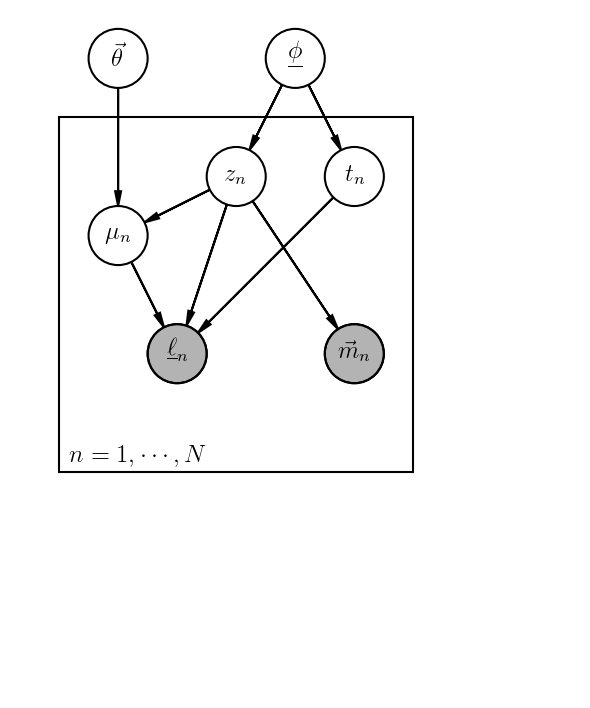
\includegraphics{Hubble-draft.png}
\caption{This directed acyclic graph corresponds to a probabilistic graphical model for our hierarchical inference of the Hubble parameter.  In this graph, all random variables are shown in circles ({\bf What is meant by "random" here?}), with observed variables shown in shaded circles.  The box indicates that there are $N$ copies of the relationships between boxed parameters, each independent of all others.  The hyperparameters we would like to infer are the cosmological parameters in $\vec{theta}$ and the supernova type-redshift distribution parameters comprising $\textul{\phi}$.  Drawn from functions of these hyperparameters are the distance moduli $\{\mu_{n}\}_{N}$, redshifts $\{z_{n}\}_{N}$, and supernova types $\{t_{n}\}_{N}$.  Here, we observe host galaxy colors $\{\vec{m}_{n}\}_{N}$ and multi-band supernova lightcurves $\{\textul{\ell}_{n}\}_{N}$, shown in shaded circles.}
\label{fig:pgm}
\end{center}
\end{figure}
\vspace{1in}

The goal here is to constrain the posterior distribution of the hyperparameters of interest given the data.

{\bf We should give a physical description of what these hyperparameters are: in this case of the Hubble Diagram we are interested in constraining the cosmology so omega matter, omega gamma, and H naut.}

We first expand this in terms of Bayes' Rule.

\begin{align}
p(\vec{\theta}, \textul{\phi} | \{\textul{\ell}_{n}\}_{N}, \{\vec{m}_{n}\}_{N}) &\propto p(\vec{\theta}, \textul{\phi})\ p(\{\textul{\ell}_{n}\}_{N}, \{\vec{m}_{n}\}_{N} | \vec{\theta}, \textul{\phi})
\end{align}

{\bf In plain English we are saying that the likelihood of a certain cosmology and the hyperparameters given some set of observed supernova lightcurves and fluxes is proportional to the prior on the cosomological parameters multiplied by the likelihood of the lightcurves and fluxes given the cosmology and hyperparameters.}

Next, we invoke the independence of the supernova parameters and observations; the $n^{th}$ system's parameters and data are assumed to be independent of the $(n+1)^{th}$ system's parameters and data.

{\bf In essence this is saying that each supernova observed is independent of every other supernova observed. Is this a safe assumption? What are the caveats of making this assumption?}

\begin{align}
p(\{\textul{\ell}_{n}\}_{N}, \{\vec{m}_{n}\}_{N} | \vec{\theta}, \textul{\phi}) &= \prod_{n}^{N}p(\textul{\ell}_{n}, \vec{m}_{n} | \vec{\theta}, \textul{\phi})
\end{align}

{\bf This assumption is necessary for us to easily combine the contributions to likelihoods of the individual supernova. Here we are saying the the likelihood of the set of lightcurves and fluxes is simply the product of each of the individual likelihoods.}

Next, we use marginalization of the latent variables, because we do not wish to estimate their values directly.

\begin{align}
p(\textul{\ell}_{n}, \vec{m}_{n} | \vec{\theta}, \textul{\phi}) &= \iiint p(\textul{\ell}_{n}, \vec{m}_{n} | \mu_{n}, z_{n}, t_{n})\ p(\mu_{n}, z_{n}, t_{n} | \vec{\theta}, \textul{\phi})\ d\mu_{n}\ dz_{n}\ dt_{n}
\end{align}

{\bf Now we expand the expression to include the latent variables, the intermediate values that are not directly measured but calculated from the measured data. In this case are latent variables are distance modulus, redshift, and type the values that we are producing in the simulated data.}

We note that the equation calls for likelihoods $\{p(\textul{\ell}_{n}, \vec{m}_{n} | \mu_{n}, z_{n}, t_{n})\}_{N}$ ({\bf the likelihood of a certain measured lightcurve and flux given some distance modulus, redshift, and type.}), but what we have are interim posteriors $\{p(\mu_{n}, z_{n}, t_{n} | \textul{\ell}_{n}, \vec{m}_{n}, \vec{\theta}^{*}, \textul{\phi}^{*})\}_{N}$ ({\bf likelihood of some distance modulus, redshift, and type given the lightcurve, flux, and the priors that are used in the fitting of the lightcurve to a suite of templates. This would be a good time to go into a discuss about how lightcurve fitters work.}) for some interim priors $\vec{\theta}^{*}, \textul{\phi}^{*}$.  The interim priors represent the beliefs about the hyperparameters $\vec{\theta}$ and $\textul{\phi}$ that go into our calculation of the posteriors from the data; whether explicitly chosen (as in methods relying on a template library) or implicitly derived (as in methods relying on a training data set), the interim priors are always present in the calculation of posterior distributions from data.  We will thus have to transform the math to be in terms of quantities we actually have.  We do this by multiplying the likelihood by an inspired factor of unity, in terms of the interim posteriors.

\begin{align}
p(\textul{\ell}_{n}, \vec{m}_{n} | \mu_{n}, z_{n}, t_{n}) &= p(\textul{\ell}_{n}, \vec{m}_{n} | \mu_{n}, z_{n}, t_{n})\ \frac{p(\mu_{n}, z_{n}, t_{n} | \textul{\ell}_{n}, \vec{m}_{n}, \vec{\theta}^{*}, \textul{\phi}^{*})}{p(\mu_{n}, z_{n}, t_{n} | \textul{\ell}_{n}, \vec{m}_{n}, \vec{\theta}^{*}, \textul{\phi}^{*})}
\end{align}

We will expand the denominator of that factor of unity according to Bayes' Rule.

\begin{align}
p(\mu_{n}, z_{n}, t_{n}|\textul{\ell}_{n}, \vec{m}_{n}, \vec{\theta}^{*}, \textul{\phi}^{*}) &= \frac{p(\mu_{n}, z_{n}, t_{n} | \vec{\theta}^{*}, \textul{\phi}^{*})\ p(\textul{\ell}_{n}, \vec{m}_{n} | \mu_{n}, z_{n}, t_{n}, \vec{\theta}^{*}, \textul{\phi}^{*})}{p(\textul{\ell}_{n}, \vec{m}_{n} | \vec{\theta}^{*}, \textul{\phi}^{*})}
\end{align}

By the independence of different hierarchical levels in the probabilistic graphical model, we may split up the most daunting term in the above expression.

\begin{align}
p(\textul{\ell}_{n}, \vec{m}_{n} | \mu_{n}, z_{n}, t_{n}, \vec{\theta}^{*}, \textul{\phi}^{*}) &= p(\textul{\ell}_{n}, \vec{m}_{n} | \mu_{n}, z_{n}, t_{n})\ p(\textul{\ell}_{n}, \vec{m}_{n} | \vec{\theta}^{*}, \textul{\phi}^{*})
\end{align}

Noting the presence of $p(\textul{\ell}_{n}, \vec{m}_{n} | \mu_{n}, z_{n}, t_{n})$ and $p(\textul{\ell}_{n}, \vec{m}_{n} | \vec{\theta}^{*}, \textul{\phi}^{*})$ in both the numerator and denominator for $p(\textul{\ell}_{n}, \vec{m}_{n} | \mu_{n}, z_{n}, t_{n})$, we cancel the like terms to express the individual likelihoods in terms of known quantities.

\begin{align}
p(\textul{\ell}_{n}, \vec{m}_{n} | \mu_{n}, z_{n}, t_{n}) &= \frac{p(\mu_{n}, z_{n}, t_{n} | \textul{\ell}_{n}, \vec{m}_{n}, \vec{\theta}^{*}, \textul{\phi}^{*})}{p(\mu_{n}, z_{n}, t_{n} | \vec{\theta}^{*}, \textul{\phi}^{*})}
\end{align}

We are now ready to plug the individual likelihoods into the marginalization.

\begin{align}
p(\textul{\ell}_{n}, \vec{m}_{n} | \vec{\theta}, \textul{\phi}) &= \iiint p(\mu_{n}, z_{n}, t_{n} | \textul{\ell}_{n}, \vec{m}_{n}, \vec{\theta}^{*}, \textul{\phi}^{*})\ \frac{p(\mu_{n}, z_{n}, t_{n} | \vec{\theta}, \textul{\phi})}{p(\mu_{n}, z_{n}, t_{n} | \vec{\theta}^{*}, \textul{\phi}^{*})}\ d\mu_{n}\ dz_{n}\ dt_{n}
\end{align}

Now we can plug the marginalization back into the product.

\begin{align}
p(\{\textul{\ell}_{n}, \vec{m}_{n}\}_{N} | \vec{\theta}, \textul{\phi}) &= \prod_{n}^{N}\ \iiint p(\mu_{n}, z_{n}, t_{n} | \textul{\ell}_{n}, \vec{m}_{n}, \vec{\theta}^{*}, \textul{\phi}^{*})\ \frac{p(\mu_{n}, z_{n}, t_{n} | \vec{\theta}, \textul{\phi})}{p(\mu_{n}, z_{n}, t_{n} | \vec{\theta}^{*}, \textul{\phi}^{*})}\ d\mu_{n}\ dz_{n}\ dt_{n}
\end{align}

And finally, we can plug the product back into Bayes' Rule.

\begin{align}
p(\vec{\theta}, \textul{\phi} | \{\textul{\ell}_{n}, \vec{m}_{n}\}_{N}) &\propto p(\vec{\theta}, \textul{\phi})\ \prod_{n}^{N}\ \iiint p(\mu_{n}, z_{n}, t_{n} | \textul{\ell}_{n}, \vec{m}_{n}, \vec{\theta}^{*}, \textul{\phi}^{*})\ \frac{p(\mu_{n}, z_{n}, t_{n} | \vec{\theta}, \textul{\phi})}{p(\mu_{n}, z_{n}, t_{n} | \vec{\theta}^{*}, \textul{\phi}^{*})}\ d\mu_{n}\ dz_{n}\ dt_{n}
\end{align}

This is the posterior we will attempt to sample!

\section{Mock Data}
\label{sec:data}

To avoid making an analysis pipeline that depends on the choice of supernova classification lightcurve fitting, and photometric redshift assignment techniques, we create mock data in the form of a catalog of $N$ interim posteriors (indexed by $n$).  To achieve the goal of simulating a mock dataset of three-dimensional posterior distributions over supernova type, redshift, and distance modulus, conditioned on interim prior values of the hyperparameters, we will have to employ a forward model.

\subsection{Choosing the true hyperparameters}
\label{sec:true_hypers}

We begin by setting true values of the hyperparameters.  $\vec{\theta}$ represents the generating cosmology of our simulation, a vector comprised of $\Omega_{\Lambda}$, $\Omega_{m}$, $H_{0}$, etc.  We choose the true cosmological parameters comprising $\vec{\theta}'$ to be those observed by [choose a well-accepted survey's results and give the elements of the vector in a table].  

$\textul{\phi}$ represents the parameters defining the supernova type proportions as a function of redshift, which we choose to be a $T\times Z$ dimensional matrix for a space with $T$ possible supernova types $\tau$ and $Z$ redshift bins $\zeta$ of widths $\vec{\Delta}_{z}$, where each element of $\phi_{\tau\zeta}$ is the probability density associated with a supernova of type $\tau$ with a redshift in bin $\zeta$; thus we have $p(z_{\zeta}, t_{\tau} | \textul{\phi}) \equiv \phi_{\zeta\tau}$, with $\textul{\phi}$ satisfying the normalization condition $\sum_{\tau=1}^{T}\textul{\phi}\cdot\vec{\Delta}_{z}=1$.  We proceed to choose a physically motivated true matrix of redshift-dependent supernova type proportions $\textul{\phi}'$.

Supernova rates are calculated by convolving the Delay time distribution with the star formation history. We then set the relative rates of SN Ia and Core Collapse to be 25\% and 75\%, respectively, at z = 0. We use the delay time distribution (DTD) for SN Ia from Graur et al (2013), the delay time distribution (DTD) for SN II from Zapartas et al (2017), and the Cosmic Star Formation Rate from Behroozi et al (2013).

\begin{figure}
	\begin{center}
		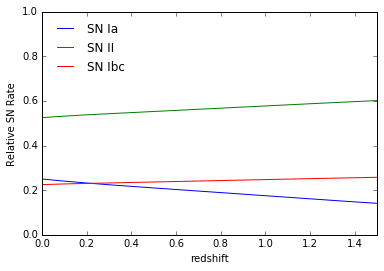
\includegraphics[width=0.95\textwidth]{relative_supernova_rate.png}
		\caption{The relative supernova rates as a function of redshift. Sums to one at every redshift.}
		\label{fig:realtive_supernova_rates}
	\end{center}
\end{figure}

\subsubsection{Supernova Type Ia Rate with Redshift}
\label{sec:TypeIaRate}

\subsubsection{Supernova Type II Rate with Redshift}
\label{sec:TypeIIRate}

To determine the rate of SNII per unit comoving volume we will basically apply the approach by Forster et al. 2006/Strogler et al. 2004 adapted to SNe II following Botticella et al. 2012.

The rate of SNe II per unit time per unit comoving volume ($R_{II}$) is given by the star formation rate ($SFR$) per unit time per unit comoving volume convolved with the number of stars crearted that will explode as SNe II.

\begin{align}
	\label{eq:rateII}
	R_{II} = K_{II} \times SFR
\end{align}

First, we must calculate the fraction of stars that explode as SN II:

\begin{align}
\label{eq:rateII}
K_{II} = \frac{\int_{m_{l,II}}^{m_{u,II}} \phi(m) \mathrm{d}m}{\int_{m_{l}}^{m_{u}} m\phi(m) \mathrm{d}m}
\end{align}

When we integrate from a minimum mass, $m_{l,II}$, of 8 to a maximum mass, $m_{u,II}$, to 25 and assuming a Salpeter et al. (1955) IMF we get a rate of $6.027 \time 10^{-3}$.

We will use three different models of how the SFR evolutions with redshift: Cole et al. (2001), Horiuchi et al. (2011), and Madau et al. (2014)

\begin{figure}
	\begin{center}
		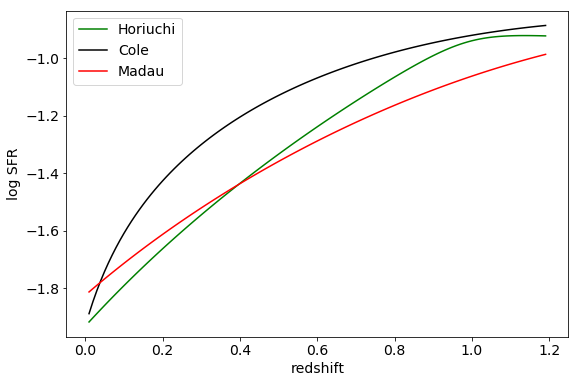
\includegraphics[width=0.95\textwidth]{SNII_SFR.png}
		\caption{SFR evolutions with redshift: Cole et al. (2001), Horiuchi et al. (2011), and Madau et al. (2014).}
		\label{fig:SNII_SFR}
	\end{center}
\end{figure}

Next we will take the spectral model of Dessart et al. (2013) which is anchored to SN II 1999em, as a reference. We simulate its $r$-band light curve at different redshifts and convolve it with the LSST filters to see when it falls below the detection limit.

\begin{figure}
	\begin{center}
		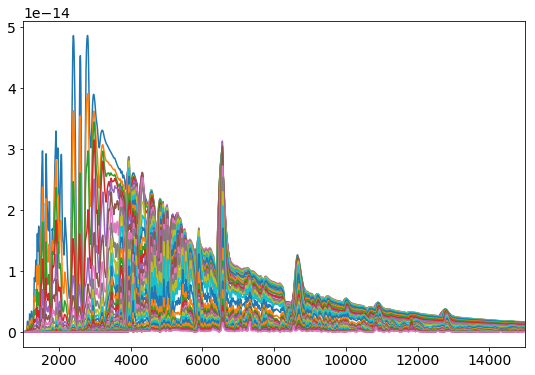
\includegraphics[width=0.95\textwidth]{spectral_model_SNII.png}
		\caption{SN II spectral model of Dessart et al. (2013): $M_{99em}=-16.6$; $M_{05J}=-17.2$}
		\label{fig:SNII_lc}
	\end{center}
\end{figure}

\begin{figure}
	\begin{center}
		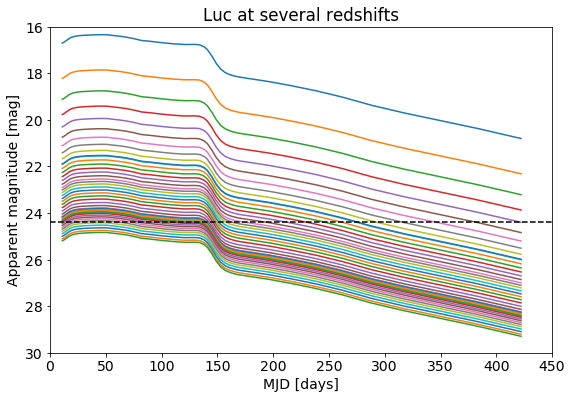
\includegraphics[width=0.95\textwidth]{SNII_lc_withz.png}
		\caption{The $r$-band lightcurve of spectral model of SN II 1999em shifted to a range of redshifts. The horizontal dashed line indicates the limiting magnitude of LSST in the $r$-band in a single visit.}
		\label{fig:SNII_lc_wz}
	\end{center}
\end{figure}

For this model SN II, we compare the magnitude as a function of time and redshift, $m(t,z)$, with the limiting magnitude, $m_{lim}$, of the LSST camera to obtain the probability of detecting (the peak of) a SN at a given redshift, $\Delta_{t}(z)$. Then we estimate the number of detected SNe II per unit of redshift, $dN/dz$, using Equations 2 and 5 of Forster et al. (2006).

\begin{figure}
	\begin{center}
		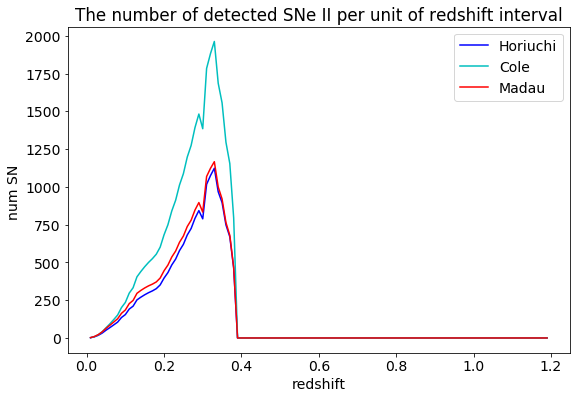
\includegraphics[width=0.95\textwidth]{number_SNII.png}
		\caption{The number of SN II detected, for each of the SFR models, as a function of redshift. The total number of SN II for Horiuchi et al. 16985, Cole et al. 29207, and Madau et al.  18322. }
		\label{fig:SNII_lc_wz}
	\end{center}
\end{figure}

Finally, we will use a a sample of 10,000 SNe, simulated using MCMC on real parameters of CSP SNe II. We will put each at 100 random redshifts from 0.01 to 1.20, so we will have 1,000,000 SNe. Now we consider the magnitude at the end of the plateau phase, instead of the peak magnitude. This is because in SN II cosmology, we do not standardize the magnitude at peak, but either the magnitude at around the center of the plateau (for spectroscopic methods), or the length/brightness-decline of the plateau (for photometric methods).

We use the apparent magnitudes at the end of the plateau phase and k-correct the magnitudes. Then we measure $\Delta_t(z)$, selecting different magnitude limit depending on the filter we use for observations. Finally, we compare the number of supernovae as a function of redshift for the three different SFR models.

\begin{figure}
	\begin{center}
		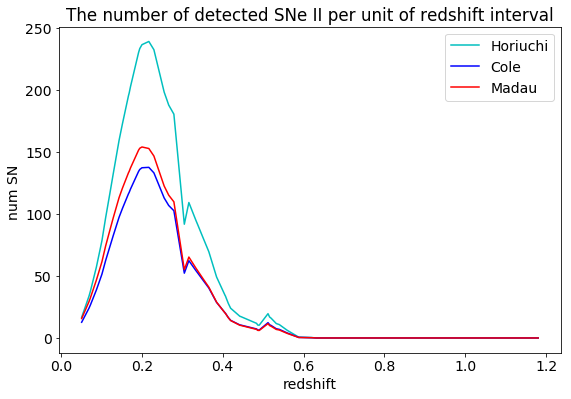
\includegraphics[width=0.95\textwidth]{number_SNII_withmagntiudescatter.png}
		\caption{The number of SN II detected, for each of the SFR models, as a function of redshift. The total number of SN II for Horiuchi et al. 16985, Cole et al. 29207, and Madau et al.  18322. }
		\label{fig:SNII_lc_wz}
	\end{center}
\end{figure}

\subsubsection{Supernova Type Ibc Rate with Redshift}
\label{sec:TypeIbcRate}
 
\subsection{Setting true values of the latent variables}
\label{sec:true_latents}

Because the redshift-dependent supernova type proportions are parametrized by $\textul{\phi}'$ such that $p(z\in\zeta, t=\tau | \textul{\phi}') = \phi_{\zeta\tau}$, it is easy to draw pairs of true types and redshifts $(t_{n}', z_{n}')$ from $\textul{\phi}'$.  We treat the elements of $\textul{\phi}'$ as a discrete distribution, noting that the redshift-dependent supernova type proportions are normalized such that $\sum_{\tau}\int_{\zeta}\textul{\phi}=1$.  Sampling the function defined by $\textul{\phi}'$ is equivalent to sampling true types and redshift bins.  Once the redshift bins have been chosen, we may choose a true redshift for each supernova from a uniform distribution defined between the bin endpoints.  This procedure gives us pairs of true types and redshifts $(t_{n}', z_{n}')$.

Finally, we calculate the true $\mu_{n}'$ according to [insert distance modulus equation from astropy.cosmology here] from $z_{n}'$ and $\vec{\theta}'$.  Rather than writing the form of the distance modulus as a function of redshift and cosmological parameters throughout the paper, we will instead use the shorthand $\mu = f_{\vec{\theta}}(z)$ here.  This results in a true catalog of length $N$ consisting of trios $(t_{n}', z_{n}', \mu_{n}')$ of the latent variables.

\subsection{Constructing PDFs}
\label{sec:pdfs}

The catalog of trios of true latent variables in the catalog must be transformed into three-dimensional probability distribution functions (PDFs) over these three variables.  We extend the binned parametrization of $\textul{\phi}$ chosen in Sec. \ref{sec:true_hypers}.  In addition to dimensions for $T$ types and $Z$ redshift bins, the PDFs have an additional dimension of $D$ distance modulus bins $\nu$ of widths $\vec{\Delta}_{\mu}$.  

Since we are aiming to construct posteriors, we know from Bayes' Rule that they will take the form of Eq. \ref{eq:mockBayes}.

\begin{align}
\label{eq:mockBayes}
p(\mu_{n}, z_{n}, t_{n} | \textul{\ell}_{n}, \vec{m}_{n}, \vec{\theta}^{*}, \textul{\phi}^{*}) &\propto p(\textul{\ell}_{n}, \vec{m}_{n} | \mu_{n}, z_{n}, t_{n}, \vec{\theta}^{*}, \textul{\phi}^{*})\ p(\mu_{n}, z_{n}, t_{n} | \vec{\theta}^{*}, \textul{\phi}^{*})
\end{align}

We will discuss the two terms separately. The first term of Eq. \ref{eq:mockBayes} may easily be reduced to $p(\textul{\ell}_{n}, \vec{m}_{n} | \mu_{n}, z_{n}, t_{n})$, as there is no direct dependence of the data on the hyperparameters.  Fig. \ref{fig:pgm} tells us how to break it up, resulting in Eq. \ref{eq:first}.

\begin{align}
\label{eq:first}
p(\textul{\ell}_{n}, \vec{m}_{n} | \mu_{n}, z_{n}, t_{n}) &= p(\textul{\ell}_{n} | \mu_{n}, z_{n}, t_{n})\ p(\vec{m}_{n} | z_{n})
\end{align}

 According to Fig. \ref{fig:pgm}, we have Eq. \ref{eq:second}.

\begin{align}
\label{eq:second}
p(\mu_{n}, z_{n}, t_{n} | \vec{\theta}^{*}, \textul{\phi}^{*}) &= p(\mu_{n} | z_{n}, \vec{\theta}^{*})\ p(z_{n}, t_{n} | \textul{\phi}^{*})
\end{align}

These two terms will be addressed separately in Secs. \ref{sec:likelihoods} and \ref{sec:posteriors}.

\subsubsection{Creating likelihoods}
\label{sec:likelihoods}

Now we are ready for a generative model of the likelihoods of lightcurves and galaxy photometry conditioned on the latent parameters.  

For each $n$, $p(\textul{\ell}_{n} | \mu_{n}, z_{n}, t_{n})$ will be a $T\times Z\times D$ three-dimensional array $\textul{L}^{n}$.  

We assume that a lightcurve classifier/fitter has been specified, and that its confusion matrix $\textul{C}$ is known.  The elements $C_{\tau'\hat{\tau}} = p(t_{n}' | \hat{t}_{n})$ of the confusion matrix represent the probability that a randomly chosen supernova of true type $t'$ is classified as type $\hat{t}$.  For all $T^{2}$ combinations of $\tau'$ and $\hat{\tau}$, there is a function $\mathcal{F}_{\tau'\hat{\tau}}(z, \mu)$ that maps pairs $(z', \mu')$ onto pairs $(\hat{z}, \hat{\mu})$, which corresponds to the output of the lightcurve fitting function when using a template of type $\hat{\tau}$ to fit a lightcurve that is truly of $\tau'$, in the absence of observational errors.  

We assume that the lightcurve fitter produces an accurate multivariate Gaussian likelihood estimate for each fit $n$ with covariance $\textul{\Sigma}$  We draw maximum likelihood values for $(\hat{z}^{\ell}, \hat{\mu}^{\ell})$ from the multivariate Gaussian distribution $\mathcal{N}_{(\hat{z}^{\ell}_{n}, \hat{\mu}^{\ell}_{n}), \textul{\Sigma}_{n}}$.  

Thus, the lightcurve likelihood may be written as $L^{n}_{\tau\zeta\nu} = C_{\tau'_{n}\tau}\mathcal{N}_{(\hat{z}^{\ell}, \hat{\mu}^{\ell}), \textul{\Sigma}_{n}}(z_{\zeta}, \mu_{\nu})$.

Next, we tackle $p(\vec{m}_{n} | z_{n})$, which will be a length $Z$ array $\vec{M}^{n}$, which is the likelihood that forms the basis for what is commonly reported as the photo-$z$ PDF $p(z_{n})$.   We will assume a very simple model for photo-$z$ likelihoods, that of a Gaussian distribution.  We draw a maximum likelihood photo-$z$ $\hat{z}_{n}^{m}$ from the distribution $\mathcal{N}_{z'_{n}, \sigma_{n}^{2}}$.  Then $M^{n}_{\zeta}=\mathcal{N}_{\hat{z}_{n}^{m}, \sigma_{n}^{2}}(z_{\zeta})$.

The overall likelihood of Eq. \ref{eq:first} is simply the product of $L^{n}_{\tau\zeta\nu}$ and $M^{n}_{\zeta}$.

\subsubsection{Making interim posteriors}
\label{sec:posteriors}

To make interim posteriors, we introduce the interim priors of Eq. \ref{eq:second}.  We choose $\vec{\theta}^{*}$ and $\textul{\phi}^{*}$ [specify what a good, general choice would be].  Because the parametrization hasn't changed, the term $p(z_{\zeta}, t_{\tau} | \textul{\phi}^{*})$ takes the simple form of $\phi^{*}_{\tau\zeta}$.  Similarly, $p(\mu_{\nu} | z_{\zeta}, \vec{\theta}^{*})$ will be a delta function $\delta_{f_{\vec{\theta}}(z_{\zeta})}(\mu_{\nu})$.  

Finally, in Eq \ref{eq:interimposteriordata}, we put these pieces together to express the form of the individual interim posteriors of the form of Eq. \ref{eq:mockBayes}.

\begin{align}
\label{eq:interimposteriordata}
p_{n}(\mu_{\nu}, z_{\zeta}, t_{\tau} | \textul{\ell}_{n}, \vec{m}_{n}, \vec{\theta}^{*}, \textul{\phi}^{*}) &= KC_{\tau'_{n}\tau}\mathcal{N}_{(\hat{z}^{\ell}, \hat{\mu}^{\ell}), \textul{\Sigma}_{n}}(z_{\zeta}, \mu_{\nu}) \mathcal{N}_{\hat{z}_{n}^{m}, \sigma_{n}^{2}}(z_{\zeta}) \phi_{\zeta\tau}\delta_{f_{\vec{\theta}}(z_{\zeta})}(\mu_{\nu})
\end{align}

The constant of proportionality $K$ here will be set such that $\sum_{\nu}^{D}\sum_{\zeta}^{Z}\sum_{\tau}^{T} p_{n}(\mu_{\nu}, z_{\zeta}, t_{\tau} | \textul{\ell}_{n}, \vec{m}_{n}, \vec{\theta}^{*}, \textul{\phi}^{*})=1$.

%\clearpage
%
%\begin{itemize}
%\item $p(z_{n}, t_{n} | \textul{\phi}^{*})$: 
%\item $p(\mu_{n} | z_{n}, \vec{\theta}^{*})$
%\item $p(\vec{m}_{n} | \mu_{n}, z_{n})$
%\item $p(\textul{\ell}_{n} | \mu_{n}, z_{n}, t_{n})$
%\end{itemize}
%
%We will first draw pairs of true parameters $(T_{n}^{0}, z_{n}^{0})$ from $p(T_{n}, z_{n} | \textul{\Phi}_{0}) = \mathcal{D}\left[\textul{\Phi}_{0}\right]$, which in this case is a discrete distribution.  Then we will calculate the true $\mu_{n}^{0}$ according to [insert distance modulus equation here] from $z_{n}^{0}$ and $\vec{\theta}_{0}$.  This may be interpreted as $p(\mu_{n} | z_{n}, \vec{\theta}) = 1$, so $p(\mu_{n}, z_{n}, T_{n} | \vec{\theta}^{*}, \textul{\Phi}^{*}) = p(z_{n}, T_{n} | \textul{\Phi}^{*}) p(\mu_{n} | z_{n}, \vec{\theta}^{*})$
%
%Next, we will construct three-dimensional likelihoods for each supernova over $\mu_{n}$, $z_{n}$, and $T_{n}$.  $\textul{\ell}_{n}$ and $\vec{f}_{n}$ are independent of one another, so we may state Eq. \ref{eq:independentdata}.
%
%\begin{align}
%\label{eq:independentdata}
%p(\textul{\ell}_{n}, \vec{f}_{n} | \mu_{n}, z_{n}, T_{n}, \vec{\theta}^{*}, \textul{\Phi}^{*})\ p(\mu_{n}, z_{n}, T_{n} | \vec{\theta}^{*}, \textul{\Phi}^{*})
%\end{align}
%
%We know $p(T_{n} | T_{n}^{0})$ as the row $\vec{r}(T_{n}^{0}) = p(T_{n} | T_{n}^{0})$ of the confusion matrix corresponding to $T_{n}^{0}$.  We denote this as the discrete distribution $p(T_{n} | T_{n}^{0}) = \mathcal{D}\left[\vec{r}(T_{n}^{0})\right]$.  In the simplest case, the redshifts are Gaussian distributions of variance $\sigma_{z}^{2}$ about $z_{n}' \sim \mathcal{N}\left[z_{n}^{0}, \sigma_{z}^{2}\right]$ for a constant $\sigma_{z}$ across the whole survey.  Thus we may write $p(z_{n} | z_{n}^{0}) = \mathcal{N}\left[z_{n}', \sigma_{z}^{2}\right]$ and $p(z_{n}, T_{n} | z_{n}^{0}, T_{n}^{0}) = p(z_{n} | z_{n}^{0}) p(T_{n} | T_{n}^{0})$.
%
%We know that $p(\mu_{n} | T_{n}, z_{n})$ will be nontrivial because 
%
%\begin{align}
%T_{n}' &\sim D[\vec{r}(T_{n})]\\
%z_{n}' &\sim \vec{\Phi}(T_{n})\\
%\mu_{n}' &= \mu(z_{n}', \vec{\theta})
%\end{align}

%\acknowledgments

%\appendix

\bibliography{references}

\end{document}